\chapter{Đại cương tổ hợp}

Chúng ta có hai quy tắc đếm, và những công thức đếm khác đều
được sinh ra cũng như tuân theo hai quy tắc này. Đó là quy
tắc cộng và quy tắc nhân.

\section{Quy tắc cộng và quy tắc nhân}

Khi một công việc có thể thực hiện bằng một trong nhiều phương án,
ta sử dụng quy tắc cộng. Ví dụ, nếu chúng ta muốn lấy một cây bút
trong hộp có 3 cây bút đỏ, 4 cây bút xanh và 5 cây bút vàng, thì
chúng ta có tất cả $3+4+5=12$ cách lấy.

Khi một công việc được thực hiện trên nhiều công đoạn, ở mỗi
công đoạn có nhiều phương án thì ta sử dụng quy tắc nhân.
Ví dụ, nếu chúng ta đi từ thành phố A tới thành phố B, giữa
đường đi ngang thành phố C. Từ A tới C có 4 con đường, từ C
tới B có 3 con đường thì có tất cả $4 \cdot 3 = 12$ con đường đi
từ A tới B mà đi ngang qua C.

\textbf{Nguyên lý bù trừ}. Ở quy tắc cộng, khi các phương án
rời nhau, thì ta cộng chúng lại. Tuy nhiên, khi các phương 
án có sự giao nhau thì chúng ta sử dụng nguyên lý bù trừ,
hay còn gọi là quy tắc cộng mở rộng.

Gọi $A$ và $B$ là hai tập hợp. Ký hiệu $\lvert A \cup B\rvert$ là
số lượng phần tử của $A$ hợp $B$ và $\lvert A \cap B \rvert$ là
số lượng phần tử của $A$ giao $B$.

Khi đó
\begin{equation}
    \lvert A \cup B \rvert = \lvert A \rvert + \lvert B \rvert
        - \lvert A \cap B \rvert
\end{equation}

Sử dụng sơ đồ Venn để mô tả công thức trên:

\begin{figure}[ht]
    \centering
    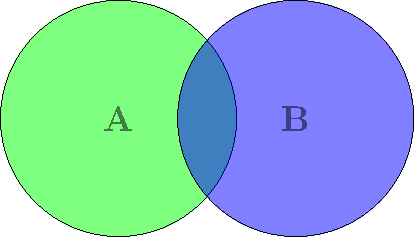
\includegraphics{../pics/set/venn1.pdf}
    \caption{Nguyên lý bù trừ cho hai tập hợp}
\end{figure}

Ta thấy rằng, khi chúng ta cộng số phần tử của hai tập hợp lại
với nhau thì phần giao của chúng bị trùng. Do đó ta phải trừ
đi một lần phần giao thì mới có hợp của hai tập hợp.

\begin{example}
    Trong một lớp học có 20 học sinh. Trong đó có 13 học sinh
    biết chơi bóng chuyền, 15 học sinh biết chơi bóng bàn. Biết
    rằng không có học sinh nào không biết chơi cả bóng chuyền lẫn
    bóng bàn. Hỏi có bao nhiêu học sinh biết chơi cả hai môn bóng
    chuyền và bóng bàn?
\end{example}

\begin{solution}
    Đặt $A$ là tập hợp các học sinh biết chơi bóng chuyền. Ta có
    $\lvert A \rvert = 13$.

    Đặt $B$ là tập hợp các học sinh biết chơi bóng bàn. Ta có
    $\lvert B \rvert = 15$.

    Do lớp học có 20 học sinh và học sinh nào cũng biết chơi
    hoặc bóng chuyền, hoặc bóng bàn, nên $\lvert A \cup B \rvert
    = 20$.

    Theo nguyên lý bù trừ, số lượng học sinh biết chơi cả hai
    bộ môn là $\lvert A \cap B \rvert = \lvert A \rvert +
    \lvert B \rvert - \lvert A \cup B \rvert = 13 + 15 - 20 = 8$.

    Như vậy có 8 học sinh biết chơi cả hai môn.
\end{solution}

Ta có thể có công thức bù trừ cho 3 tập hợp.
\begin{equation}
    \lvert A \cup B \cup C \rvert = \lvert A \rvert + \lvert B \rvert
    + \lvert C \rvert - (\lvert A \cap B \rvert + \lvert B \cap C \rvert
    + \lvert C \cap A \rvert) + \lvert A \cap B \cap C \rvert
\end{equation}

Trong trường hợp tổng quát cho $n$ tập hợp $A_1$, $A_2$, ..., $A_n$
thì công thức bù trừ là:

\begin{equation}
\begin{split}
    \lvert A_1 \cup A_2 \cup \ldots \cup A_n \rvert & =
    \sum_{i=1}^{n} \lvert A_i \rvert \\ - & \sum_{1 \leq i_1, i_2, \leq n
    , i_1 \neq i_2} \lvert A_{i_1} \cap A_{i_2} \rvert \\
    + & \sum_{1 \leq i_1, i_2, i_3, i_1 \neq i_2 \neq i_3 \neq i_1}
    \lvert A_{i_1} \cap A_{i_2} \cap A_{i_3} \rvert + \ldots \\ + 
    & (-1)^{t-1} \sum_{1 \leq i_1, \ldots, i_t, i_1 \neq \ldots \neq i_t}
    \lvert A_{i_1} \cap \ldots \cap A_{i_t} \rvert + \ldots \\ +
    & (-1)^{n-1} \lvert A_1 \cap \ldots \cap A_n \rvert
\end{split}
\end{equation}

\section{Hoán vị, tổ hợp, chỉnh hợp}

Xét một tập hợp $n$ phần tử
\[A = \{a_1, a_2, \ldots, a_n\}\]

Một cách xếp $n$ phần tử này theo thứ tự là một hoán vị của tập
hợp đó. Tập hợp có $n$ phần tử thì số hoán vị là $n!$.

\begin{proof}
    Xét vị trí đầu tiên, ta có thể xếp một trong $n$ phần tử
    vào vị trí này. Đối với vị trí thứ hai, vì ta đã xếp 
    một phần tử vào vị trí đầu nên ta còn $n-1$ phần tử có thể
    xếp vào vị trí thứ hai. Tương tự, với vị trí thứ ba ta có
    $n-2$ cách chọn. Cho tới vị trí cuối cùng (vị trí thứ $n$)
    ta còn đúng 1 phần tử.

    Do đó, theo quy tắc nhân, số cách xếp $n$ phần tử theo thứ
    tự là \[n \cdot (n-1) \cdot (n-2) \cdots 2 \cdot 1 = n!\]
\end{proof}

Ví dụ, với tập $A = \{1, 2, 3\}$ thì ta có các hoán vị là 
$\{1, 2, 3\}$, $\{1, 3, 2\}$, $\{2, 1, 3\}$, $\{2, 3, 1\}$,
$\{3, 1, 2\}$ và $\{3, 2, 1\}$.

Chỉnh hợp là một trường hợp nhỏ hơn của hoán vị. Khi đó từ
một tập hợp có $n$ phần tử, ta lấy ra $k$ phần tử và sắp 
$k$ phần tử đó theo thứ tự. Khi đó với $k \leq n$ thì số
chỉnh hợp là $\dfrac{n!}{(n-k)!}$.

\begin{proof}
    Vị trí đầu tiên ta có $n$ cách chọn. Vị trí thứ 2 ta có
    $n-1$ cách chọn. Tương tự vậy, ta thấy rằng ở vị trí
    thứ $i$ thì ta có $n-i+1$ cách chọn (chỉ số của vị trí
    và số cách chọn luôn có tổng bằng $n+1$).

    Do đó, tới vị trí thứ $k$ thì số cách chọn là $n-k+1$.
    Như vậy theo quy tắc nhân, số chỉnh hợp là
    \begin{equation}
        \begin{split}
            & n \cdot (n-1) \cdots (n-k+1) \\ = & \frac{
         n \cdot (n-1) \cdots (n-k+1) \cdot (n-k) \cdot (n-k-1) 
         \cdots 2 \cdot 1}
        {(n-k) \cdot (n-k-1) \cdots 2 \cdot 1} \\ 
        = & \frac{n!}{(n-k)!}
        \end{split}
    \end{equation}
\end{proof}

Khi chúng ta lấy ra $k$ phần tử từ $n$ phần tử nhưng không
sắp chúng theo thứ tự, ta có tổ hợp. Do đó ta cần chia cho
số hoán vị của $k$ phần tử. Như vậy số tổ hợp $k$ phần tử
từ tập hợp $n$ phần tử là $\dfrac{n!}{(n-k)! \cdot k!}$.